\documentclass[tikz,border=10pt]{standalone}
\begin{document}

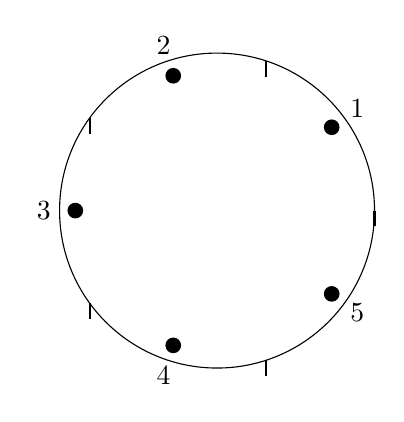
\begin{tikzpicture}[scale=2]

% Draw the circle
\draw (0,0) circle (1);

% Divide the circle into five equal parts
\foreach \i in {0,72,...,324} {
    \draw[thick] (\i:1) -- ++(0,-0.1);
}

% Label the arcs with numbers
\node at (36:1.1) {1};
\node at (108:1.1) {2};
\node at (180:1.1) {3};
\node at (252:1.1) {4};
\node at (324:1.1) {5};

% Indicate the positions of the effective vertices (black dots)
\node[fill=black,circle,inner sep=2pt] at (36:0.9) {};
\node[fill=black,circle,inner sep=2pt] at (108:0.9) {};
\node[fill=black,circle,inner sep=2pt] at (180:0.9) {};
\node[fill=black,circle,inner sep=2pt] at (252:0.9) {};
\node[fill=black,circle,inner sep=2pt] at (324:0.9) {};

\end{tikzpicture}

\end{document}